%!TEX root = ../../main.tex

\chapter{Das Monty-Hall-Problem}

\section{Einführung}

Das Monty-Hall-Problem (oft auch als Ziegenproblem bezeichnet) ist Statistikern als Paradoxon in der Elementarwahrscheinlichkeitstheorie bekannt.
Es geht dabei um die Frage, ob eine Wahl, die zunächst zufällig unter drei a priori gleich wahrscheinlichen Möglichkeiten getroffen wurde, geändert werden sollte, wenn zusätzliche Informationen enthüllt werden.
\begin{wrapfigure}{r}{0.3\textwidth}
    \centering
    \captionsetup{name=Abb., justification=centering, format=nolinebreak}
    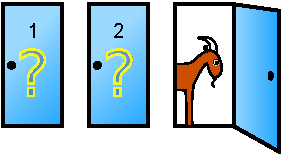
\includegraphics{Monty_open_door.pdf}
    \caption{das Monty-Hall-Problem} \label{fig:monty-hall}
    \small Nachdem der Kandidat das erste Tor gewählt hat öffnet der Moderator Tor 3. Nun steht der Kandidat vor der Wahl: soll er bei seiner ersten Wahl bleiben oder auf Tor 3 wechseln?
\end{wrapfigure}
Die Aufgabe ist ursprünglich aus der von Monty Hall modertierten Spielshow ,,Lets Make a Deal'' abzuleiten. Sie fand ihren Anfang
1963 und ihr Ende 1977. In jeder Folge spielte der Moderator der Spielshow, Monty Hall, Spiele mit seinem Publikum. Diese Spiele variierten stark, jedoch war das Grundprinzip
häufig das Selbe. Spieler aus dem Publikum mussten sich zwischen garantierten, kleinen Gewinnen und eventuellen, durch ,,Glückspiel'' gewonnene, große Preise, entscheiden.
In einer der Folgen, die häufig als die Klimax der Show beschrieben wird, wurde den Spielern aus dem Publikum drei identische Türen gezeigt. Hinter diesen drei
identischen Türen befinden sich die potenziellen Gewinne, wovon zwei Gewinne Ziegen waren. Hinter der dritten Tür war jedoch der Hauptgewinn, ein neues Auto.

Das Problem, wie es heutzutage unter Mathematikern bekannt ist, wurde ursprünglich als Leserbrief an Marilyn vos Savant\footnote{Vos Savant hat laut dem Guinness Buch der Rekorde den höchsten jemals gemessenen IQ.} in ihrer Kolumne \textit{Ask Marilyn} im Magazin Parade veröffentlicht:

\begin{quote}
    Nehmen Sie an, Sie wären in einer Spielshow und hätten die Wahl zwischen drei Toren. Hinter einem der Tore ist ein Auto, hinter den anderen sind Ziegen. Sie wählen ein Tor, sagen wir, Tor Nummer 1, und der Showmaster, der weiß, was hinter den Toren ist, öffnet ein anderes Tor, sagen wir, Nummer 3, hinter dem eine Ziege steht. Er fragt Sie nun: ,,Möchten Sie das Tor Nummer 2?'' Ist es von Vorteil, die Wahl des Tores zu ändern? (\cite{Savant:1990})
\end{quote}

Dieses Problem, wie es auch in \autoref{fig:monty-hall} dargestellt ist, zeigt, wie die intuitive Wahrnehmung von Wahrscheinlichkeiten von der tatsächlichen Mathematik abweichen kann. Selbst unter Mathematikern wurde das Problem und vor allem die von vos Savant vorgestellte Lösung stark diskutiert und kritisiert\footnote{wie wir später sehen werden nicht ganz zu Unrecht}.

\section{Möglichkeiten des Kandiaten}

Grundlegend hat der Kandidat zwei Mögichkeiten nachdem der Moderator ein Ziegentor geöffnet hat: Wechseln oder nicht wechseln. Die Meisten, die sich vorher noch nicht mit diesem Problem beschäftigt haben, werden intuitiv denken, dass sie hier eine Gewinnwahrscheinlichkeit von $50\%$ haben, egal ob sie wechseln oder nicht. Andere denken womöglich, der Moderator möchte einem dazu bringen, die Auswahl zu ändern, da sie mit ihrer ersten Wahl richtig lagen.

\subsection{Wechseln oder nicht ist egal}

Zu diesem Schluss kommen die Meisten, wenn sie sich das erste Mal mit diesem Problem auseinandersetzen. Sie gehen davon aus, dass sie nun eine Gewinnwahrscheinlichkeit von $50\%$ haben, egal wie sie sich entscheiden.

\subsection{Bei der ersten Wahl bleiben}

Geht man davon aus, bei beiden Toren die gleiche Gewinchance zu haben, entscheiden sich die Meisten dafür, bei ihrer ersten Wahl zu bleiben. Dies lässt sich damit erklären, dass man von einer einmaligen Spielsituation ausgeht (im Leserbrief wurde auch nichts anderes erwähnt) und man nichts über die Motivation des Moderators weiß. Wenn man schon einige Spielshows gesehen hat, denkt man möglicherweiße aus Erfahurung, der Moderator wolle einen nur verunsichern und von der ersten richtigen Wahl abbringen.\footnote{Dass die meisten bei ihrer Ursprünglichen Wahl bleiben, wurde genauer in der Dokuserie ,,Mythbusters'' (Staffel 9, Episode 21) untersucht und bestätigt.}

\subsection{Auf jeden Fall wechseln}

Nur die wenigsten treffen diese Wahl.


